\documentclass[12pt]{article}
\usepackage[a4paper, total={6in, 8in}]{geometry}
\usepackage{amsfonts}
\usepackage{amsmath,amssymb,trimclip,adjustbox}
\usepackage{breqn}
\usepackage{pgfplots}
\usepackage{hyperref}
\usepackage{tabularray}
\usepackage{polski}
\usepackage[utf8]{inputenc}

\setlength{\parindent}{0pt}
\setlength{\textheight}{650pt}
\setlength{\oddsidemargin}{0pt}
\setlength{\textwidth}{480pt}

\hypersetup{
    colorlinks=true,
    linkcolor=blue,
    filecolor=magenta,      
    urlcolor=cyan,
    pdftitle={Overleaf Example},
    pdfpagemode=FullScreen,
}

\author{Michał Puchyr}
\title{Sprawozdanie 100B}

\begin{document}
\maketitle

\section{Cel ćwiczenia}

\begin{itemize}
    \item Pomiar rezystancji na opornikach oraz żarówce
    \item Zmierzenie wartości napięcia i natężenia na opornikach oraz żarówce
    \item Obliczenie oporu przy pomocy praw fizyki i porównanie go z wcześniejszymi pomiarami
    \item Zrozumienie praw fizyki związanych z prądem elektrycznym
\end{itemize}

\section{Opis ćwiczenia}
\subsection{Wstęp teoretyczny}

W obwodach prądu stałego rezystancja jest wielkością charakteryzującą relację między napięciem
a natężeniem prądu elektrycznego. Oznacza to, że opór przewodnika elektrycznego jest 
wprost proporcjonalny do napięcia i odwrotnie proporcjonalny do natężenia.

\label{ohm}
$$ R = \frac{U}{I} $$ 
Gdzie :

$R$ - rezystancja [$\Omega$]

$U$ - napięcie między końcami przewodnika [$V$]

$I$ - natężenie prądu elektrycznego[$A$]\\

Przyrządy i materiały wykorzystane do pomiarów : 
\begin{itemize}
    \item 2 mierniki uniwersalne M8906
    \item Zasilacz stabilizowany
    \item Przewody elektryczne
    \item Zestaw oporników z żarówką
\end{itemize}

\pagebreak

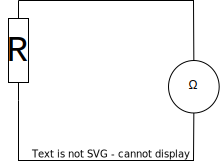
\includegraphics{obwod1.pdf}

Schemat układu nr 1 - do wyznaczenia rezystancji każdego z oporników
za pomocą omomierza

\includegraphics{obwod2.pdf}

Schemat układu nr 2 - do wyznaczenia napięcia i natężenia na opornikach za pomocą
amperomierza i woltomierza

\section{Pomiary układów}

\begin{tabular}{ |p{0.5cm}|p{2cm}|p{3cm}|p{3cm}|p{3cm}| }
    \hline
    \multicolumn{5}{|c|}{Pomiary oporu w układzie pierwszym} \\
    \hline
    Lp. &Opornik & Niepewność[$\Omega$] & Zakres[$\Omega$] & Opór [$\Omega$] \\ 
    \hline
    1 & $R_1$ & 1,0 & 200 & 165,20  \\
    2 && 1,0 & 200 & 165,30 \\
    3 && 1,0 & 200 & 164,90 \\
    4 && 1,0 & 200 & 165,00 \\
    \hline
    5& $R_2$ & 0,8 & 200 & 122,60\\
    6&& 0,8 & 200 & 122,90 \\
    7&& 0,8 & 200 & 123,00 \\
    8&& 0,8 & 200 & 122,90 \\
    \hline
    9& Żarówka & 0,3 & 200 & 13,90 \\
    10&& 0,3 & 200 & 13,80\\
    11&& 0,3 & 200 & 13,90\\
    12&& 0,3 & 200 & 13,90\\
    \hline
\end{tabular}

\begin{adjustbox}{center}
\begin{tabular}{|p{0.5cm}|p{1.5cm}|p{1cm}|p{1.5cm}|p{1.5cm}|p{2cm}|p{1.3cm}|p{1.2cm}|p{1.5cm}|p{1.5cm}|}
    
    \hline
    \multicolumn{10}{|c|}{Pomiary napięcia i natężenia w układzie drugim} \\
    \hline
    Lp. & Opornik& U[$V$]& u(U)[V] & I[$10^{-3}A$] & u(I)[$10^{-3}A$] & R[$\Omega$] & $U_c[\Omega]$ & R śr.[$\Omega$] & u($\overline{R}$)[$\Omega$] \\ 
    \hline
    1 & $R_1$ & 3,210 & 0,020 & 19,50 & 0,20 & 164,7 & 1,9 & 163,97 & 0,09\\
    2 && 4,660 & 0,020 & 28,40 & 0,26 & 164,1& 1,7 && \\
    3 && 6,190 & 0,020& 37,70& 0,32 & 164,2& 1,6 && \\
    4 && 7,700 & 0,030& 47,00& 0,39 & 163,9& 1,5 && \\
    5 && 9,340 & 0,030& 57,10& 0,46 & 163,6& 1,5&& \\
    6 && 6,190 & 0,020& 37,80& 0,32 & 163,8& 1,6&& \\
    7 && 4,650 & 0,020& 28,40& 0,26 & 163,8& 1,7&& \\
    8 && 3,210 & 0,020& 19,60& 0,20 & 163,8& 1,9&& \\
    9 && 7,700 & 0,030& 47,00& 0,39 & 163,9& 1,5&& \\
    10 && 9,340 & 0,030 & 57,00 & 0,46 & 163,9& 1,5&& \\
    \hline
    11 & $R_2$ & 3,200 & 0,020 & 26,20 & 0,24 & 122,2 & 1,3 & 122,11 & 0,05 \\
    12 && 4,630 & 0,020 & 37,90 & 0,33 & 122,2& 1,2 && \\
    13 && 6,160 & 0,020 & 50,40 & 0,41 & 122,3& 1,1 && \\
    14 && 7,660 & 0,030 & 62,80 & 0,50 & 122,0& 1,1 && \\
    15 && 9,290 & 0,030 & 76,20 & 0,59 & 122,0& 1,1 && \\
    16 && 3,190 & 0,020 & 26,20 & 0,24 & 121,8& 1,3 && \\
    17 && 4,630 & 0,020 & 37,90 & 0,33 & 122,2& 1,2 && \\
    18 && 6,160 & 0,020 & 50,40 & 0,41 & 122,3& 1,1 && \\
    19 && 7,650 & 0,030 & 62,70 & 0,50 & 122,1& 1,1 && \\
    20 && 9,290 & 0,030 & 76,20 & 0,59 & 122,0& 1,1 && \\
    \hline
    21 & Żarówka & 3,160 & 0,020 & 43,50 & 0,36 & 72,7 & 0,7 & 93,89 & 4,68 \\
    22 && 4,600 & 0,020 & 54,40 & 0,44 & 84,6& 0,8  && \\
    23 && 6,130 & 0,020 & 63,70 & 0,50 & 96,3& 0,9  && \\
    24 && 7,640 & 0,030 & 73,00 & 0,57 & 104,7& 0,9  && \\
    25 && 9,280 & 0,030 & 82,70 & 0,64 & 112,3& 1,0  && \\
    26 && 3,160 & 0,020 & 43,50 & 0,36 & 72,7& 0,7   &&\\
    27 && 4,600 & 0,020 & 54,40 & 0,44 & 84,6& 0,8   &&\\
    28 && 6,130 & 0,020 & 64,60 & 0,51 & 94,9& 0,9  && \\
    29 && 7,640 & 0,030 & 73,70 & 0,57 & 103,7& 0,9  && \\
    30 && 9,280 & 0,030 & 82,60 & 0,64 & 112,4& 1,0 && \\
    \hline
\end{tabular}
\end{adjustbox}\\

Rezystancja w układzie drugim została obliczona przy użyciu \hyperlink{ohm}{prawa Ohma}.
Pomiary zostały wykonane przy zakresie 200mA i 20V.

\subsection{Wykres I = f(U)}

\subsubsection{Wykres dla pomiaru opornika R1}
\includegraphics{pomiar1.png}

\subsubsection{Wykres dla pomiaru opornika R2}
\includegraphics{pomiar2.png}

\subsubsection{Wykres dla pomiaru żarówki}
\includegraphics{pomiar3.png}

\subsection{Wyznaczenie oporu przy pomocy regresji liniowej}
Wzory:

$$ R = \frac{1}{a} $$

(Regresja liniowa została wyznaczona dla miliamperów stąd wynik należy pomnożyć przez 1000)\\

Dla opornika R1 : 

$ R = \frac{1}{6,1157} \cdot 1000 = 163,57 \Omega $

Dla opornika R2 :

$ R = \frac{1}{8,206} \cdot 1000 = 121,86 \Omega $

Dla żarówki : 

$ R = \frac{1}{6,3573} \cdot 1000 = 157,29 \Omega $

\pagebreak

\section{Obliczenia}
\subsection{Niepewność typu A}

Do obliczenia niepewności pomiarowej typu A został wykorzystany poniższy wzór

$$ u_a(x) = \sqrt{\frac{\sum\limits_{i=1}^{n}(x_i - \overline{x})^2}{n(n - 1)}} $$
$$ \overline{x} = \frac{1}{n}\sum\limits_{i = 1}^{n}x_i $$

Przykładowe obliczenia (dla pierwszego opornika z pomiaru drugiego) : 

$$ \overline{x} = \frac{1}{10} \cdot (164,7 + 164,1 + 164,2 + 163,9 + 163,6 + 163,8 + 163,8 
+ 163,8 + 163,9 + 163,9 ) = 163,97 $$

$$ u_a(x) = \sqrt{\frac{\sum\limits_{i=1}^{n}(x_i - 163,92)^2}{10(10 - 1)}}
= \sqrt{\frac{0,84}{90}} = 0,09 $$

Dla pierwszego opornika : 

$ \overline{x} = 163,97\Omega $

$ u_a(x) = 0,09\Omega $\\

Dla drugiego opornika : 

$ \overline{x} = 122,11\Omega $

$ u_a(x) = 0,05\Omega $\\

Dla żarówki : 

$ \overline{x} = 93,89\Omega $

$ u_a(x) = 4,68\Omega $

\subsection{Niepewność typu B}

Do obliczenia niepewności pomiaru napięcia (zakres 20V) przez miernik wykorzystano wzór
$$ \pm 0.5\% rdg + 1dgt  $$
Do obliczenia niepewności pomiaru natężenia (zakres 200mA) przez miernik wykorzystano wzór
$$ \pm 1.2\% rdg + 1dgt  $$
Do obliczenia niepewności pomiaru oporu (zakres 200$\Omega$) przez miernik wykorzystano wzór
$$ \pm 0.8\% rdg + 3dgt  $$

Przykładowe obliczenia dla napięcia i natężenia :

$$ u(U) = 3,21 \cdot 0.5\% + 0,01 = 0,02605 \approx 0,026 $$

$$ u(I) = 19,50 \cdot 1.2\% + 0,01 = 0,244 \approx 0,25 $$

Aby wyliczyć niepewność typu B ostatecznie trzeba podzielić niepewność przez $ \sqrt{3} $

$$ u_b(U) = \frac{0,02605}{\sqrt{3}} = 0,015 \approx 0,02 $$

$$ u_b(I) = \frac{0,244}{\sqrt{3}} = 0,14 \approx 0,2 $$

Przykładowe obliczenie niepewności oporu :

$$ u(R) = 165,20 \cdot 0.8\% + 3 \cdot 0,1 = 1,62 \approx 1,7 $$

$$ u_b(R) = \frac{1,62}{\sqrt{3}} = 0,935 \approx 1,0 $$

\subsection{Niepewność typu C}

Do obliczenia tej niepewności dla danego pomiaru wykorzystano wzór

$$ u_c(R) = \sqrt{(\frac{\partial f}{\partial U})^2 u(U)^2 + (\frac{\partial f}{\partial I})^2 u(I)^2 } $$

$$ u_c(R) = \sqrt{(\frac{1}{I})^2 u(U)^2 + (\frac{-U}{I^2})^2 u(I)^2 } $$

Przykładowe obliczenie :

$$ u_c(R) = \sqrt{(\frac{1}{0,0195})^2 \cdot 0,02^2 + (\frac{-3,21}{0,0195^2})^2 \cdot 0,0002^2} = 1,88 \approx 1,9 $$

\section{Wnioski}
Poprzez wykonanie pomiarów natężenia i napięcia w układach można zauważyć, że napięcie i natężenie
w opornikach
zwiększają się proporcjonalnie względem siebie co wynika z \hyperlink{ohm}{prawa Ohma}. Poprzez
pomiar pierwszy i porównanie wyników pomiaru drugiego można zaobserwować identyczność (z małymi
odchyleniami) zmierzonego oporu z tym obliczonym przy pomocy wzoru. \\
Żarówka ze względu na zmienność temperatury nie zastosowuje się do prawa Ohma, opór zmieniał się 
w zależności od wielkości napięcia i natężenia nieliniowo. Opór zmierzony na żarówce jest znacząco
różniący się od tego, wyliczonego przy pomocy \hyperlink{ohm}{prawa Ohma}.

\section{Bibliografia}
\begin{itemize}
    \item \url{https://pl.wikipedia.org/wiki/Prawo_Ohma}
\end{itemize}

\end{document}